\section{Acción del Viento - CIRSOC 102/94}
 
Hallar las acciones del viento para un Gimnasio ubicado en la ciudad de Puerto Madryn, la zona de emplazamiento es alejado de la zona costera. Realizar el cálculo según CIRSOC 102/94. Las medidas se muestran en la siguiente figura:\\

\begin{figure}[H]
\begin{center}
     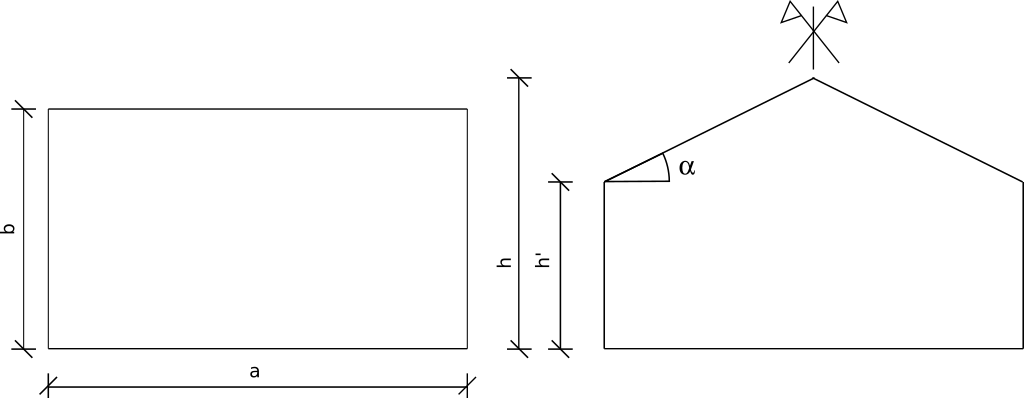
\includegraphics[scale = 0.7]{chapters/chapter_2/images/uno.png}
\end{center}
\end{figure}

\begin{align*}
& a=60m \\
& b=25m \\
& h'=7m \\
& h=10.20m \\
& \alpha=14.35\textsuperscript{o} \\
\end{align*}

Plantear todas las combinaciones de cargas de acuerdo a la reglamentación, de las acciones del peso propio, sobrecarga y viento.

\newpage
\begin{enumerate}
\item Se determina la Velocidad de referencia $\beta$ para la localidad de Puerto Madryn.\\

	\begin{center}
		$\beta=35 \frac{m}{s}$ de tabla 1 y la figura 4
	\end{center}

\item Cálculo de la Velocidad básica de diseño $V_0$.\\
Se calculara mediante la expresión:

$$V_0=C_p \cdot \beta$$

donde $C_p=1.65$ es el coeficiente de velocidad probable, que toma en consideración el riesgo y el tiempo de riesgo adoptado para la construcción de acuerdo con el tipo y destino de la misma, se obtiene de la tabla 2.

$$V_0=1.65 \cdot 35 \frac{m}{s} = 57.75 \frac{m}{s}$$

\item Cálculo de la presión dinámica básica $q_0$.\\
La presión dinámica básica es:

	\begin{align*}
	& q_0=0.000613 \cdot {V_0}^2 \\
	& q_0=0.000613 \cdot {\Big(57.75 \frac{m}{s}\Big)}^2=2.04 \frac{KN}{m^2} \Rightarrow 204.4 \frac{Kg}{m^2}
	\end{align*}

\item Cálculo de la presión dinámica de cálculo $q_z$.\\
La presión dinámica de cálculo es:

$$q_z=q_0 \cdot C_z \cdot C_d$$

donde $C_z$ es el coeficiente adimensional que expresa la ley de variación de la presión con la altura y tiene en cuenta la condición de rugosidad del terreno.\\
y $C_d$ es el coeficiente adimensional de reducción  que tiene en cuenta las dimensiones de la construcción.\\

\begin{itemize}
\item El coeficiente $C_z$ se calcula mediante:



$$C_z= \Bigg[\frac{ln\frac{z}{z_{0i}}} {ln\frac{10}{z_{01}}}\Bigg]^2 \cdot \Bigg(\frac{z_{0i}}{z_{01}}\Bigg)^{0.1412}$$

En donde:\\
$z:$ es la altura del punto considerado, respecto al nivel de referencia, en metros.\\
$z_{0i}:$ es un parámetro que depende del tipo de rugosidad del terreno.\\
$z_{01}:$ es un parámetro que corresponde al tipo de rugosidad I.\\

\newpage

De la tabla 3 obtenemos un $z_{0i}=0.005$ para rugosidad tipo I.

$$C_z= \Bigg[\frac{ln\frac{10.20m}{0.005}} {ln\frac{10}{0.005}}\Bigg]^2 \cdot \Bigg(\frac{0.005}{0.005}\Bigg)^{0.1412} = 1.0052$$

\item El coeficiente $C_d$ se obtiene mediante la tabla 5, es función de la relación $\frac{a}{h}$, $\frac{b}{h}$, $\frac{h}{V_0}$ y el tipo de rugosidad.\\

\underline{Viento según \emph{\textbf{a}} y entrando a tabla 5}
\[ 
\left \{
  \begin{tabular}{ccc}
  $\frac{a}{h} = \frac{60m}{10.20m} = 5.88$ \\
  $\frac{h}{V_0} = \frac{10.20m}{57.75 \frac{m}{s}} = 0.176$ \\
  Rugosidad Tipo I
  \end{tabular}
\right \} \Rightarrow C\textsubscript{d} = 1
\]

\begin{align*}
& q_{za}= q_0 \cdot C_z \cdot C_d \\
& q_{za}= 204.4 \frac{Kg}{m^2} \cdot 1.0052 \cdot 1 = 205.46 \frac{Kg}{m^2}
\end{align*}

\underline{Viento según \emph{\textbf{b}} y entrando a tabla 5}
\[ 
\left \{
  \begin{tabular}{ccc}
  $\frac{b}{h} = \frac{25m}{10.20m} = 2.45$ \\
  $\frac{h}{V_0} = \frac{10.20m}{57.75 \frac{m}{s}} = 0.176$ \\
  Rugosidad Tipo I
  \end{tabular}
\right \} \Rightarrow C\textsubscript{d} = 1
\]

\begin{align*}
& q_{zb}= q_0 \cdot C_z \cdot C_d \\
& q_{zb}= 204.4 \frac{Kg}{m^2} \cdot 1.0052 \cdot 1 = 205.46 \frac{Kg}{m^2}
\end{align*}

\end{itemize}

\item Relación de dimensiones $\lambda$.\\
Para una dirección del viento dada, la relación de dimensiones $\lambda$ es el cociente entre la altura \emph{\textbf{h}} y la dimensión horizontal de la cara expuesta. Según sea la cara expuesta a la acción del viento tendremos:\\

\begin{align*}
& \lambda_a = \frac{h}{a} = \frac{10.20m}{60m} = 0.17
& \lambda_b = \frac{h}{b} = \frac{10.20m}{25m} = 0.40
\end{align*}

\item Determinación del coeficiente de forma $\gamma_0$.\\
Según la ubicación de la construcción con respecto al suelo tendremos $\gamma_0$ ó $\gamma_h$ ó $\gamma_e$\\.
El coeficiente de forma $\gamma_0$ se obtiene según la dirección \emph{\textbf{a}} y \emph{\textbf{b}} a partir de la figura 13.\\

\underline{Viento normal a la cara mayor $S_a$ y entrando a la figura 13}.\\

Con $ \lambda_a < 0.5 $ y $ \lambda_b = 0.40 \Rightarrow \gamma_{0a} = 0.93$

\underline{Viento normal a la cara menor $S_b$ y entrando a la figura 13}.\\

Con $ \lambda_b < 1 $ y $ \lambda_a = 0.17 \Rightarrow \gamma_{0b} = 0.85$

\newpage
\item Permeabilidad $\mu$. \\
Si $\mu \leq 5\% \Rightarrow $ Construcción con pared cerrada.\\
Si $\mu \geq 35\% \Rightarrow $ Construcción con paredes abiertas.\\
Si $\mu > 5\%$ y $\mu \leq 35\% \Rightarrow $ Construcción con paredes parcialmente abiertas.\\
En nuestro caso debido a que el gimnasio no posee grandes aberturas se considera $\mu \leq 5\% \Rightarrow $ Construcción con pared cerrada.\\

\textbf{\underline{Cálculo como Construcción con Paredes Cerradas:}}\\
\newline
\underline{Viento según A} $\Rightarrow \gamma_{0a}=0.93 \quad \text{y} \quad \mu \leq 5\%$\\

\item Determinación de las acciones exteriores $C_e$.\\
Los valores de los coeficientes de presión exterior $C_e$ se obtienen de las tablas 6 y 7. Estos valores corresponden a un viento que no atraviesa la construcción, cuando esto no se cumple, ciertos coeficientes pueden dejar de ser válidos.\\
\begin{itemize}
	\item Barlovento	
		\begin{itemize}
		\item Pared $\Rightarrow \framebox{+0.8} $ de Tabla 6.
        \item Cubierta $\Rightarrow \framebox{-0.35} $ de la Figura 17)a) con $\alpha = 14.35\textsuperscript{o}$ y $\gamma_{0a}=0.93$
		\end{itemize}
	\item Sotavento
		\begin{itemize}
		\item Pared $\Rightarrow -(1.3 \cdot \gamma_{0a}-0.8) = \framebox{-0.409}$ de Tabla 6.
        \item Cubierta $\Rightarrow \framebox{-0.27} $ de la Figura 17)a) con $\alpha = 14.35\textsuperscript{o}$ y $\gamma_{0a}=0.93$
		\end{itemize}
	\item Paredes Laterales $\Rightarrow \framebox{-0.4} $ de la Figura 16) con $\alpha = 0\textsuperscript{o} $ y $\gamma_{0a}=0.93$
\end{itemize}

\item Determinación de las acciones interiores $C_i$.\\
Los valores de los coeficientes de presión interior $C_i$ se obtienen de la tabla 8, de conformidad con las características de la construcción, permeabilidad de las paredes y su disposición con respecto a la dirección del viento.\\
\\
$ C_i = + 0.6 \cdot (1.8 -1.3 \cdot \gamma_{0a}) = \framebox{+0.35} $ de Tabla 8.\\
\\
$ C_i = - 0.6 \cdot (1.3 \cdot \gamma_{0a} - 0.8) = \framebox{-0.24} $ de Tabla 8.\\

\newpage
\begin{figure}[H]
\begin{center}
     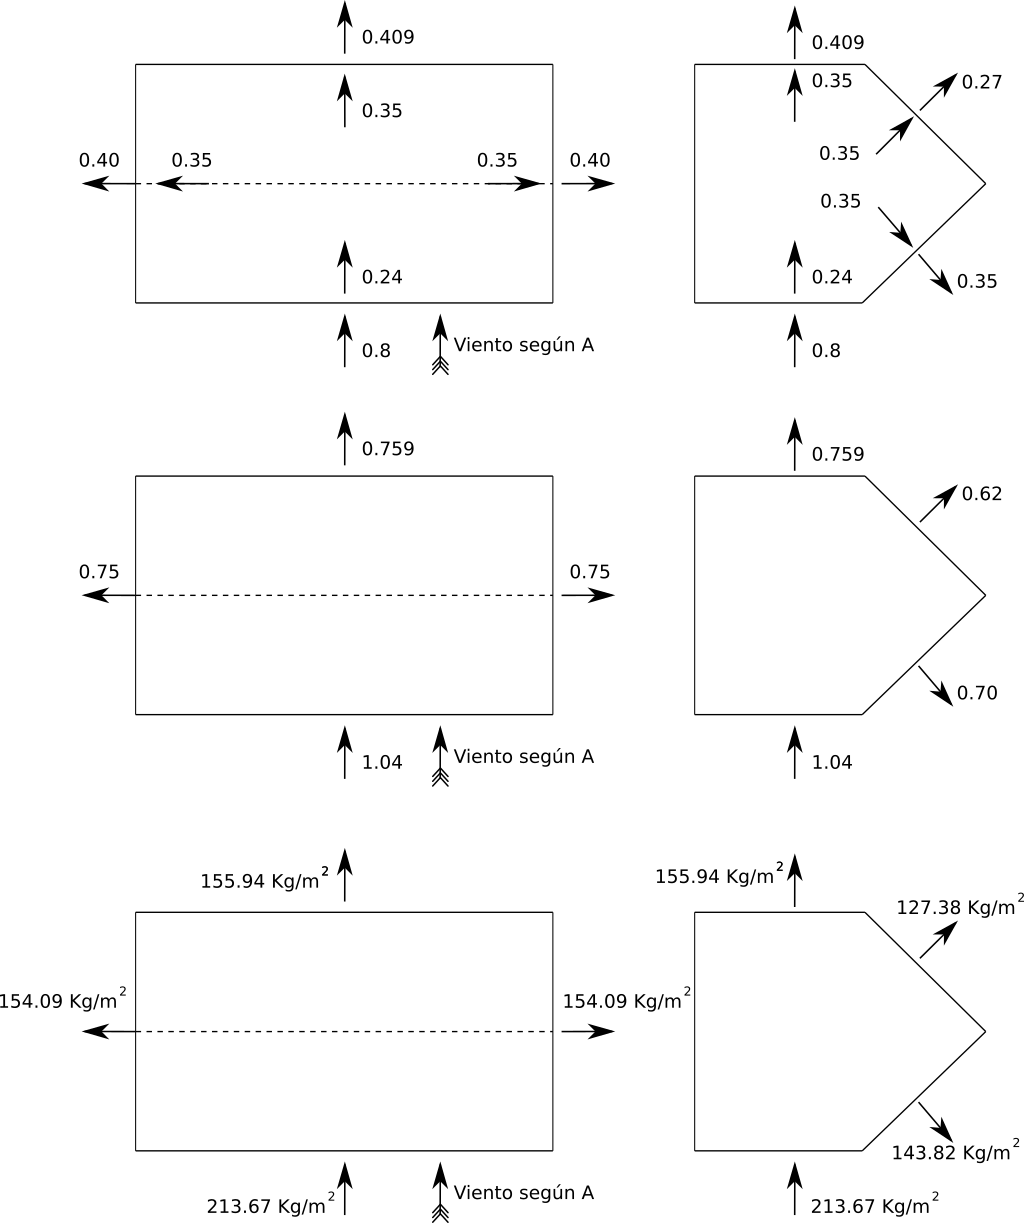
\includegraphics[scale = 0.8]{chapters/chapter_2/images/cerrada_A.png}
\end{center}
\end{figure}
\newpage


\underline{Viento según B} $\Rightarrow \gamma_{0b}=0.85 \quad \text{y} \quad \mu \leq 5\%$\\

\item Determinación de las acciones exteriores $C_e$.\\
Los valores de los coeficientes de presión exterior $C_e$ se obtienen de las tablas 6 y 7. Estos valores corresponden a un viento que no atraviesa la construcción, cuando esto no se cumple, ciertos coeficientes pueden dejar de ser válidos.\\
\begin{itemize}
	\item Barlovento	
		\begin{itemize}
		\item Pared $\Rightarrow \framebox{+0.8} $ de Tabla 6.
		\end{itemize}
	\item Sotavento
		\begin{itemize}
		\item Pared $\Rightarrow -(1.3 \cdot \gamma_{0b}-0.8) = \framebox{-0.305}$ de Tabla 6.
		\end{itemize}
	\item Paredes Laterales $\Rightarrow \framebox{-0.3} $ de la Figura 16) con $\alpha = 0\textsuperscript{o} $ y $\gamma_{0b}=0.85$
    \item Cubierta $\Rightarrow \framebox{-0.28} $ de la Figura 17)a) con $\alpha = 0\textsuperscript{o} $ y $\gamma_{0b}=0.85$
\end{itemize}

\item Determinación de las acciones interiores $C_i$.\\
Los valores de los coeficientes de presión interior $C_i$ se obtienen de la tabla 8, de conformidad con las características de la construcción, permeabilidad de las paredes y su disposición con respecto a la dirección del viento.\\
\\
$ C_i = + 0.6 \cdot (1.8 -1.3 \cdot \gamma_{0b}) = \framebox{+0.42} $ de Tabla 8.\\
\\
$ C_i = - 0.6 \cdot (1.3 \cdot \gamma_{0b} - 0.8) = -0.18 \Rightarrow \framebox{-0.20} $ de Tabla 8.\\

\newpage
\begin{figure}[H]
\begin{center}
     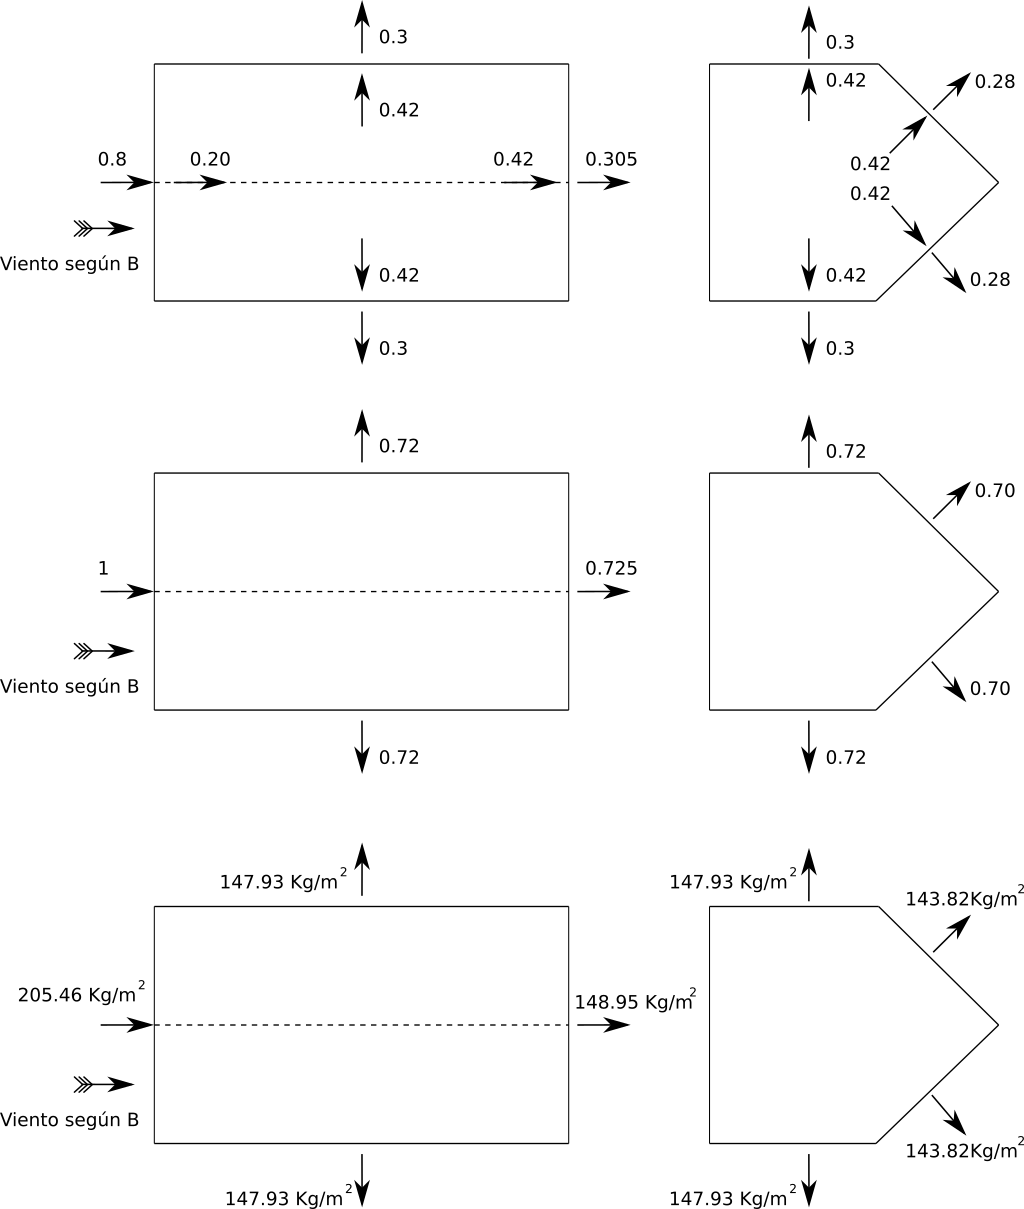
\includegraphics[scale = 0.8]{chapters/chapter_2/images/cerrada_B.png}
\end{center}
\end{figure}

\newpage
\textbf{\underline{Combinaciones de Estados de Carga}} \\
\\
$g =$ Peso propio\\
$p =$ Sobrecarga\\
$W_a =$ Viento según A\\
$W_b =$ Viento según B\\
\begin{enumerate}
    \item $g+p$
    \item $g+W_a$
    \item $g+W_b$
\end{enumerate}

\end{enumerate}